\section{随伴関手}\label{chap-9-adjoint-functor}
\begin{define}[随伴関手]\label{def-adjoint-functor}
  ある二つの関手$\functor{L}{C}{D}$、$\functor{R}{D}{C}$が随伴関手であるとは、以下の性質を満たす時である。
  \begin{quote}
    \begin{mydescription}
      \item[単位と余単位]ある自然変換$\nat{\eta}{Id_\cat{C}}{R\circ L}$と$\nat{\epsilon}{L\circ R}{Id_\cat{D}}$が存在する。また$\eta$を単位、$\epsilon$を余単位と呼ぶことにする。
      \item[三角恒等式]
      自然変換の二等式
      \[(\epsilon\circ L)\cdot(L\circ \eta)=ID_L\]
      \begin{center}
        \begin{tikzpicture}[auto]
          \node (L1) at (0, 0) {$L$};
          \node (L2) at (2, -2) {$L$};
          \node (LRL) at (2, 0) {$LRL$};

          \draw[double,double equal sign distance,-implies] (L1) -- node[swap] {$ID_L$} (L2);
          \draw[double,double equal sign distance,-implies] (L1) -- node {$L\circ \eta$} (LRL);
          \draw[double,double equal sign distance,-implies] (LRL) -- node {$\epsilon\circ L$} (L2);
        \end{tikzpicture}
      \end{center}
      \[(R\circ \epsilon)\cdot (\eta\circ R)=ID_R\]
      \begin{center}
        \begin{tikzpicture}[auto]
          \node (L1) at (0, 0) {$R$};
          \node (L2) at (2, -2) {$R$};
          \node (LRL) at (2, 0) {$RLR$};

          \draw[double,double equal sign distance,-implies] (L1) -- node[swap] {$ID_R$} (L2);
          \draw[double,double equal sign distance,-implies] (L1) -- node {$\eta\circ R$} (LRL);
          \draw[double,double equal sign distance,-implies] (LRL) -- node {$L\circ \epsilon$} (L2);
        \end{tikzpicture}
      \end{center}
      が成り立つ。
    \end{mydescription}
  \end{quote}
  また$\functor{L}{C}{D}$が左随伴関手、$\functor{R}{D}{C}$が対応する右随伴関手である時、$L\dashv R$と表記する
\end{define}

\begin{prop}[随伴関手の同値な定義]\label{prop-equivalent-definition-of-adjoint-functors}
  $L\vdash R\iff \arset{D}{LC}{D}\cong\arset{C}{C}{RD}$であり$C,D$に対して自然
\end{prop}
\begin{proof}[$\Longrightarrow$]
  任意の対象$C,D$に対して、射$\mor{\phi}{\arset{D}{LC}{D}}{\arset{C}{C}{RD}}$を
  \[\phi = \arset{C}{\eta_C}{RD}\circ R_{LC,D}\]
  と定義する。また逆射として$\mor{\phi^{-1}}{\arset{C}{C}{RD}}{\arset{D}{LC}{D}}$を
  \[\phi^{-1}=\arset{D}{LC}{\epsilon_D}\circ L_{C,RD}\]と定義する。
  \begin{center}
    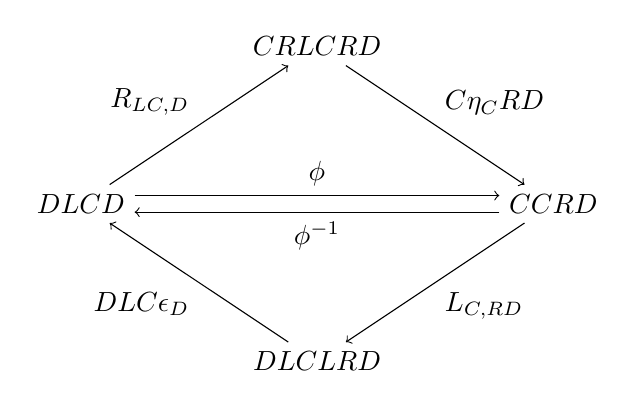
\begin{tikzpicture}[auto]
      \node (LCD) at (0, 0) {$\arset{D}{LC}{D}$};
      \node (RLCRD) at (3, 2) {$\arset{C}{RLC}{RD}$};
      \node (LCLRD) at (3, -2) {$\arset{D}{LC}{LRD}$};
      \node (CRD) at (6, 0) {$\arset{C}{C}{RD}$};
      \draw[->] (LCD) to node{$R_{LC,D}$}(RLCRD);
      \draw[->,transform canvas={yshift=3pt}] (LCD) to node{$\phi$}(CRD);
      \draw[->,transform canvas={yshift=-3pt}] (CRD) to node{$\phi^{-1}$}(LCD);

      \draw[->] (RLCRD) to node{$\arset{C}{\eta_C}{RD}$}(CRD);
      \draw[->] (LCLRD) to node{$\arset{D}{LC}{\epsilon_D}$}(LCD);
      \draw[->] (CRD) to node{$L_{C,RD}$}(LCLRD);
    \end{tikzpicture}
  \end{center}
  ただし、$R_{LC,D}$と$L_{C,RD}$は関手$R,L$の射関数の成分の一つとする。

  これが実際に同型射になることを示す。
  任意の射$\mor{f}{LC}{D}$に対して
  \begin{align*}
    (\phi^{-1}\circ\phi)(f)&=\epsilon_D\circ LRf\circ L\eta_C&\text{(展開)}\\
    &=f\circ \epsilon_{LC}\circ L\eta_C&\text{($\eta$の自然性)}\\
    &=f\circ(\epsilon L\cdot L\eta)_C&\text{(自然変換の水平合成)}\\
    &=f\circ(ID_L)_C&\text{(随伴の三角不等式)}\\
    &=f
  \end{align*}
  同様に任意の射$\mor{g}{C}{RD}$に対して
  \begin{align*}
    (\phi\circ\phi^{-1})(f)
    &=R\epsilon_D\circ RLg \circ\eta_C&\text{(展開)}\\
    &=R\epsilon_D\circ\eta_{RD}\circ g&\text{($\eta$の自然性)}\\
    &=(R\epsilon\cdot\eta R)_D\circ g&\text{(自然変換の水平合成)}\\
    &=(ID_R)_D\circ g&\text{(随伴の三角不等式)}\\
    &=g
  \end{align*}
  よって$\arset{D}{LC}{D}\cong\arset{C}{C}{RD}$である。次にこの同型の自然性を示そう。また対象$C,D$に対する同型射$\phi$を$\phi_{C,D}$と表記する。
  すなわち、$\mor{f}{C'}{C},\ \mor{g}{D}{D'}$に対して、\[\arset{C}{f}{Rg}\circ\phi_{C,D}=\phi_{C',D'}\circ\arset{D}{Lf}{g}\]
  \begin{center}
    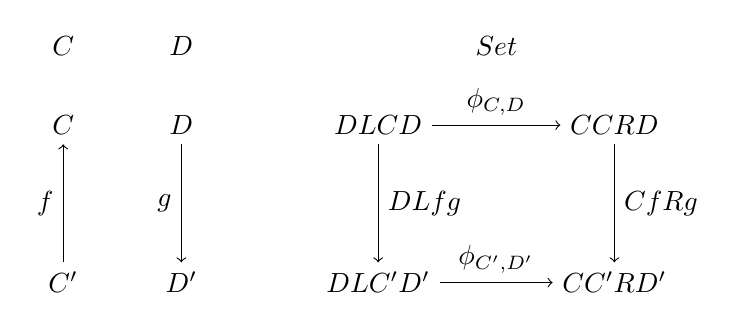
\begin{tikzpicture}[auto]
      \node (C) at (0, 2) {$C$};
      \node (C') at (0, 0) {$C'$};
      \node (catC) at (0, 3) {$\cat{C}$};

      \node (D) at (1.5, 2) {$D$};
      \node (D') at (1.5, 0) {$D'$};
      \node (catD) at (1.5, 3) {$\cat{D}$};

      \node (LCD) at (4, 2) {$\arset{D}{LC}{D}$};
      \node (LCD') at (4, 0) {$\arset{D}{LC'}{D'}$};
      \node (CRD) at (7, 2) {$\arset{C}{C}{RD}$};
      \node (CRD') at (7, 0) {$\arset{C}{C'}{RD'}$};
      \node (catD) at (5.5, 3) {$\cat{Set}$};

      \draw[->] (C') to node{$f$}(C);
      \draw[->] (D) to node[swap]{$g$}(D');
      \draw[->] (LCD) to node{$\arset{D}{Lf}{g}$}(LCD');
      \draw[->] (CRD) to node{$\arset{C}{f}{Rg}$}(CRD');
      \draw[->] (LCD) to node{$\phi_{C,D}$}(CRD);
      \draw[->] (LCD') to node{$\phi_{C',D'}$}(CRD');
    \end{tikzpicture}
  \end{center}
  を示せば良い。任意の射$\mor{h}{LC}{D}$を適用してそれぞれ展開すると、
  \begin{align*}
    (\arset{C}{f}{Rg}\circ\phi_{C,D})(h)&=Rg\circ Rh\circ\eta_C\circ f\\
    (\phi_{C',D'}\circ\arset{D}{Lf}{g})(h)&=Rg\circ Rh\circ RLf\circ \eta_{C'}
  \end{align*}
  となるが、$\eta$の自然性$\eta_C\circ f=RLf\circ \eta_{C'}$により、\[\arset{C}{f}{Rg}\circ\phi_{C,D}=\phi_{C',D'}\circ\arset{D}{Lf}{g}\]は確かに成り立つ。よって$\arset{D}{LC}{D}\cong\arset{C}{C}{RD}$が自然同型であることを示せた。
\end{proof}
\begin{proof}[$\Longleftarrow$]
  \[\eta_C = \phi_{C,LC}(id_{LC}),\ \epsilon_D=\phi^{-1}_{RD,D}(id_{RD})\]とする。これがそれぞれ単位、余単位になるか調べれば良い。
  まずはこれらが自然変換であるかを調べる。
  任意の$C$において$\arset{D}{LC}{LC}\cong\arset{C}{C}{RLC}$であり、$C$に対して自然であるから自然同型$\arset{\funccat{C}{D}}{L}{L}\cong\arset{\funccat{C}{C}}{Id}{RL}$が成り立つ。
\end{proof}
